\documentclass[ru]{./../../common/SurferDesc}%%%%%%%%%%%%%%%%%%%%%%%%%%%%%%%%%%%%%%%%%%%%%%%%%%%%%%%%%%%%%%%%%%%%%%%
%
% The document starts here:
%
\begin{document}
\footnotesize
% WeltrekordflŠchen

%%% 1.Tafel

%%%%%%%%%%%%%%%%%%%%%%%%%%%%%

\begin{surferPage}
  \begin{surferTitle}Двойной конус\end{surferTitle}  \\
Как говорилось во введении к этой галерее, поверхность называется несингулярной, если она, образно говоря, не имеет «заострений», называемых сингулярностями, например, сфера, тор (изображение 1 или 2 слева): 
    \begin{center}
      \vspace{-0.3cm}
      \begin{tabular}{@{}c@{}c@{}c@{}c@{}}
        \begin{tabular}{@{}c}
          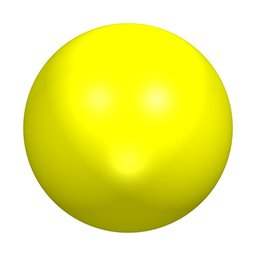
\includegraphics[width=1.4cm]{./../../common/images/kugel}
        \end{tabular}
        &
        \begin{tabular}{@{}c}
          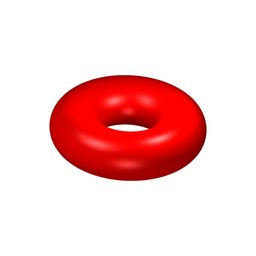
\includegraphics[width=1.4cm]{./../../common/images/torus}
        \end{tabular}
        &
        \begin{tabular}{c@{}}
          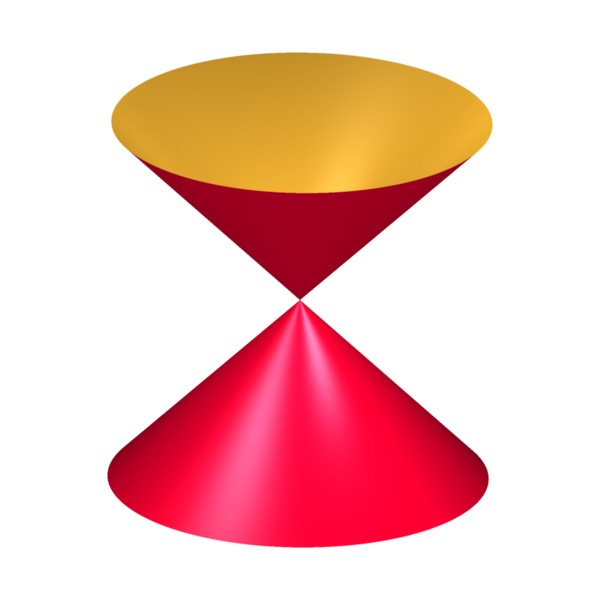
\includegraphics[width=1.4cm]{./../../common/images/kegel}
        \end{tabular}
      \end{tabular}
    \end{center}
    \vspace{-0.3cm}
Двойной конус (правое изображение) – самая простая сингулярность; она – единственная, которую можно описать уже уравнением второй степени: 
    \[x^2+y^2-z^2=0.\]
    Если его немного изменить, приписав с правой стороны уравнения величину $a\neq 0$, то он превращается в зависимости от знака §$a$ в одно- или двуполостный гиперболоид:

%    \dontshow{
    % 
    \begin{center}
      \vspace{-0.2cm}
      \begin{tabular}{@{}c@{\ }c@{\ }c@{\ }c@{\ }c@{}}
        \begin{tabular}{@{}c@{}}
          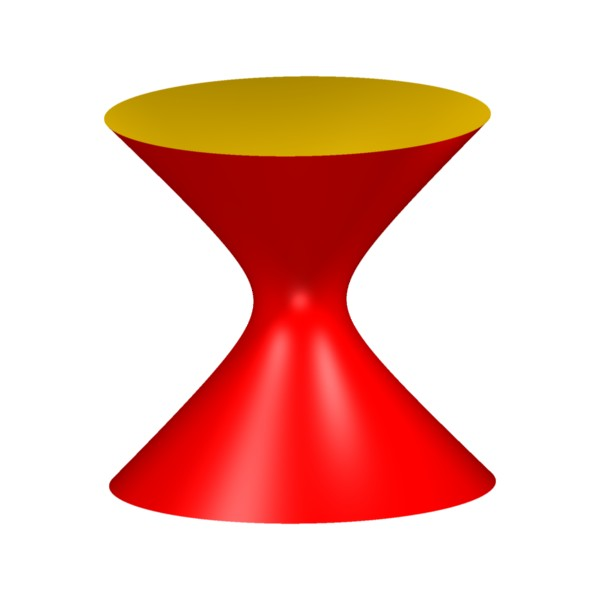
\includegraphics[width=1.2cm]{./../../common/images/A1pm_2}
        \end{tabular}
        &
        $\leftarrow$
        &
        \begin{tabular}{@{}c@{}}
          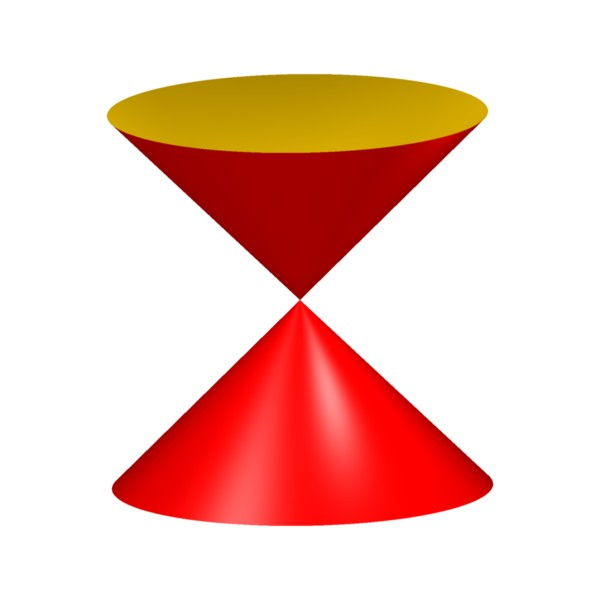
\includegraphics[width=1.2cm]{./../../common/images/A1pm_1} 
        \end{tabular}
        &
        $\rightarrow$
        &
        \begin{tabular}{@{}c@{}}
          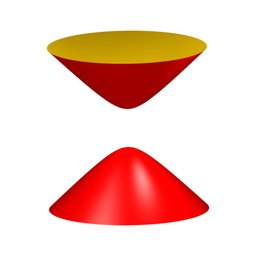
\includegraphics[width=1.2cm]{./../../common/images/A1pm_0}
        \end{tabular}
      \end{tabular}
    \end{center}
%    }
    \vspace{-0.2cm}
Поверхность второй степени имеет максимум одну сингулярность, т.е. $\mu(2)=1$.



  \begin{surferText}
     \end{surferText}
\end{surferPage}

%%%%%%%%%%%%%%%%%%%%%%


\end{document}
%
% end of the document.
%
%%%%%%%%%%%%%%%%%%%%%%%%%%%%%%%%%%%%%%%%%%%%%%%%%%%%%%%%%%%%%%%%%%%%%%%
